\documentclass[12pt]{jreport}
\usepackage{suthesis}
\usepackage[dvipdfm]{graphicx}
\graphicspath{{figs/}}
\DeclareGraphicsExtensions{.pdf,.jpg}

\thesis{
\bf 2020年度 \ \ 
%
% select one of the following
卒業論文・修士論文
}

\title{
\bf 卒業論文・修士論文の正しい\\
書き方に関する説明
}

\professor{
\begin{tabular}[t]{lr}
アサノ デービッド & 教授
\end{tabular}
}

\date{
2021年1月31日提出
}

\author{
信州大学 工学部 電子情報システム工学科 \\     
17T2000A・19W2000A \\
信州 太郎 \\
}

\begin{document}
\maketitle
\maegaki

\begin{jabstract}
    この論文でやったことを簡単に説明するところです。あらましは論文と独立に読むため、論文
    を読んでいない人でも論文の内容が大体わかるように書くこと。論文の内容とかぶってもいい。
    構成は論文の目的、提案方式、主な結果にする。

    表紙とあらましはページ番号がない。次のページのページ番号が「iii」になり、そのあとは
    「iv,v,vi,...」と続く。
\end{jabstract}

\maetsuke
\tableofcontents
\listoffigures
\listoftables

\hombun

\chapter{序論}
研究の背景、目的を書く。

各章の名称は適切に変更してもよい。

このページからページ番号が「1,2,3,...」に変更する。

参考文献は必ず本文から参照すること。例えば次のように。

過去に類似した○○の研究があり、いいことを提案した\cite{ref1}\cite{ref2}.
また、\cite{ref3}では、すごいことを証明した。

\chapter{背景技術}
論文の内容を理解するために必要な知識について書く。
節等の番号に注意すること。

章のタイトルは例であり、適切なタイトルに変更しても良い。

\section{必要知識1}
説明を書く。

\subsection{必要知識1の1}
細かくわける必要があるとき。

図\ref{fig:pm1}に図のサンプルがある。PDFにして保存するときれいになる。
JPEG等の画像フォーマットを使うと線や文字が汚くなる。

% 図はPDFで作りましょう!
\begin{figure}[htb]
    \begin{center}
        % サイズはそのまま
        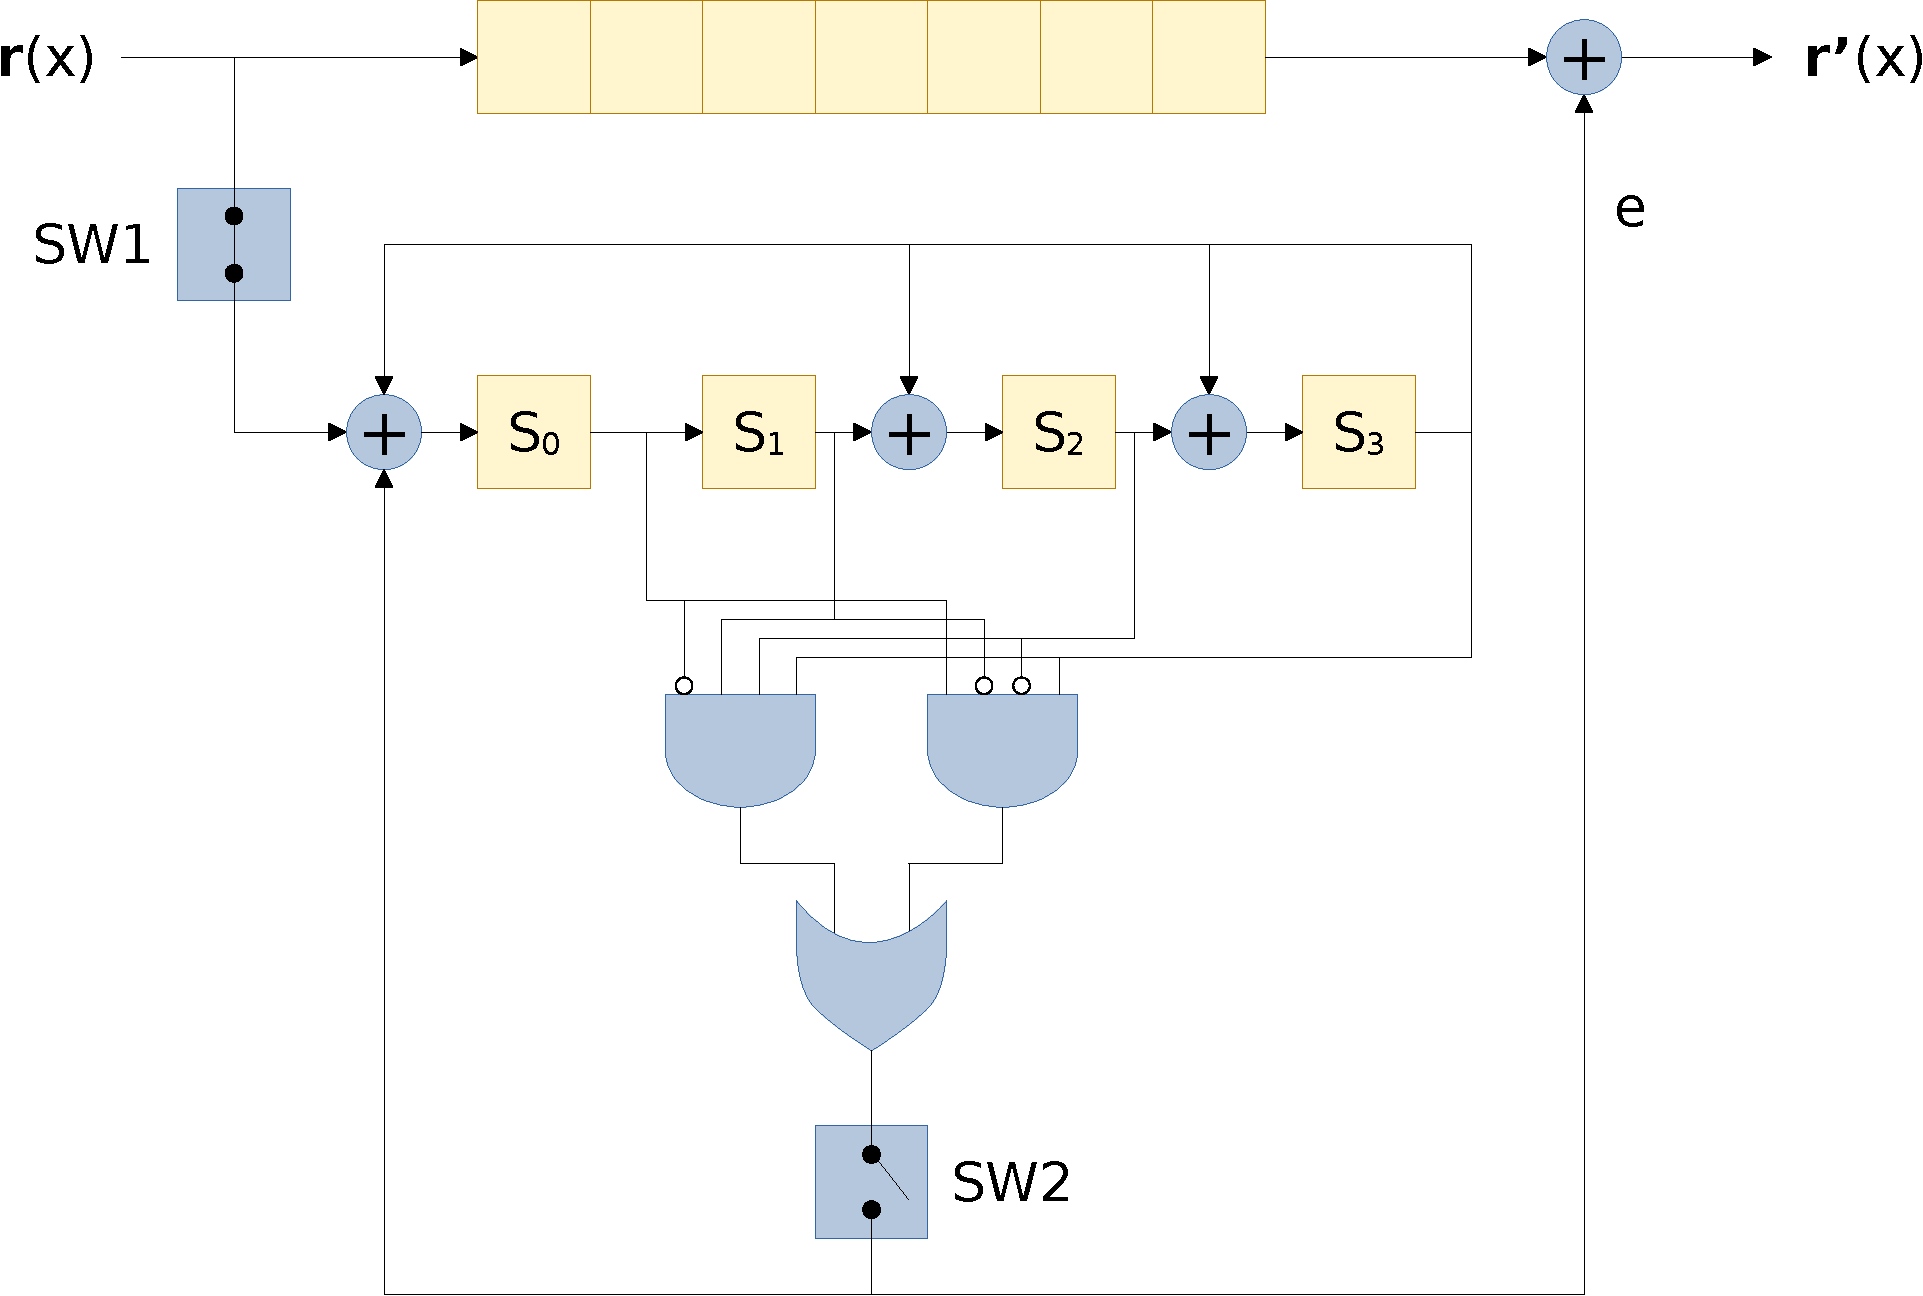
\includegraphics[width=12cm,height=8cm]{decode7_4_10111_no_margin-crop.pdf}
    \end{center}
    \caption{図のサンプル
        \label{fig:pm1}
    }
\end{figure}

図は必ず本文から参照すること。図番号に注意すること。
「章番号.章の中の連番」の形式にすること。
図の見出しは図の下に配置する。

\chapter{システムの説明}
この章では、システムの概要と機能を説明してから、実際にどう実現したかを説明する。
2章の技術も参考にしながら、全体構成からそれぞれの部分の詳細説明に移る。
システムの実際の画面等を使わずに、原理やアルゴリズムを説明する。使い方はここでは書かないこと。

図\ref{fig:pm2}に写真のサンプルがある。JPEGにして保存しよう。

% 写真はJPG
\begin{figure}[htb]
    \begin{center}
        % 幅・高さを指定する場合
        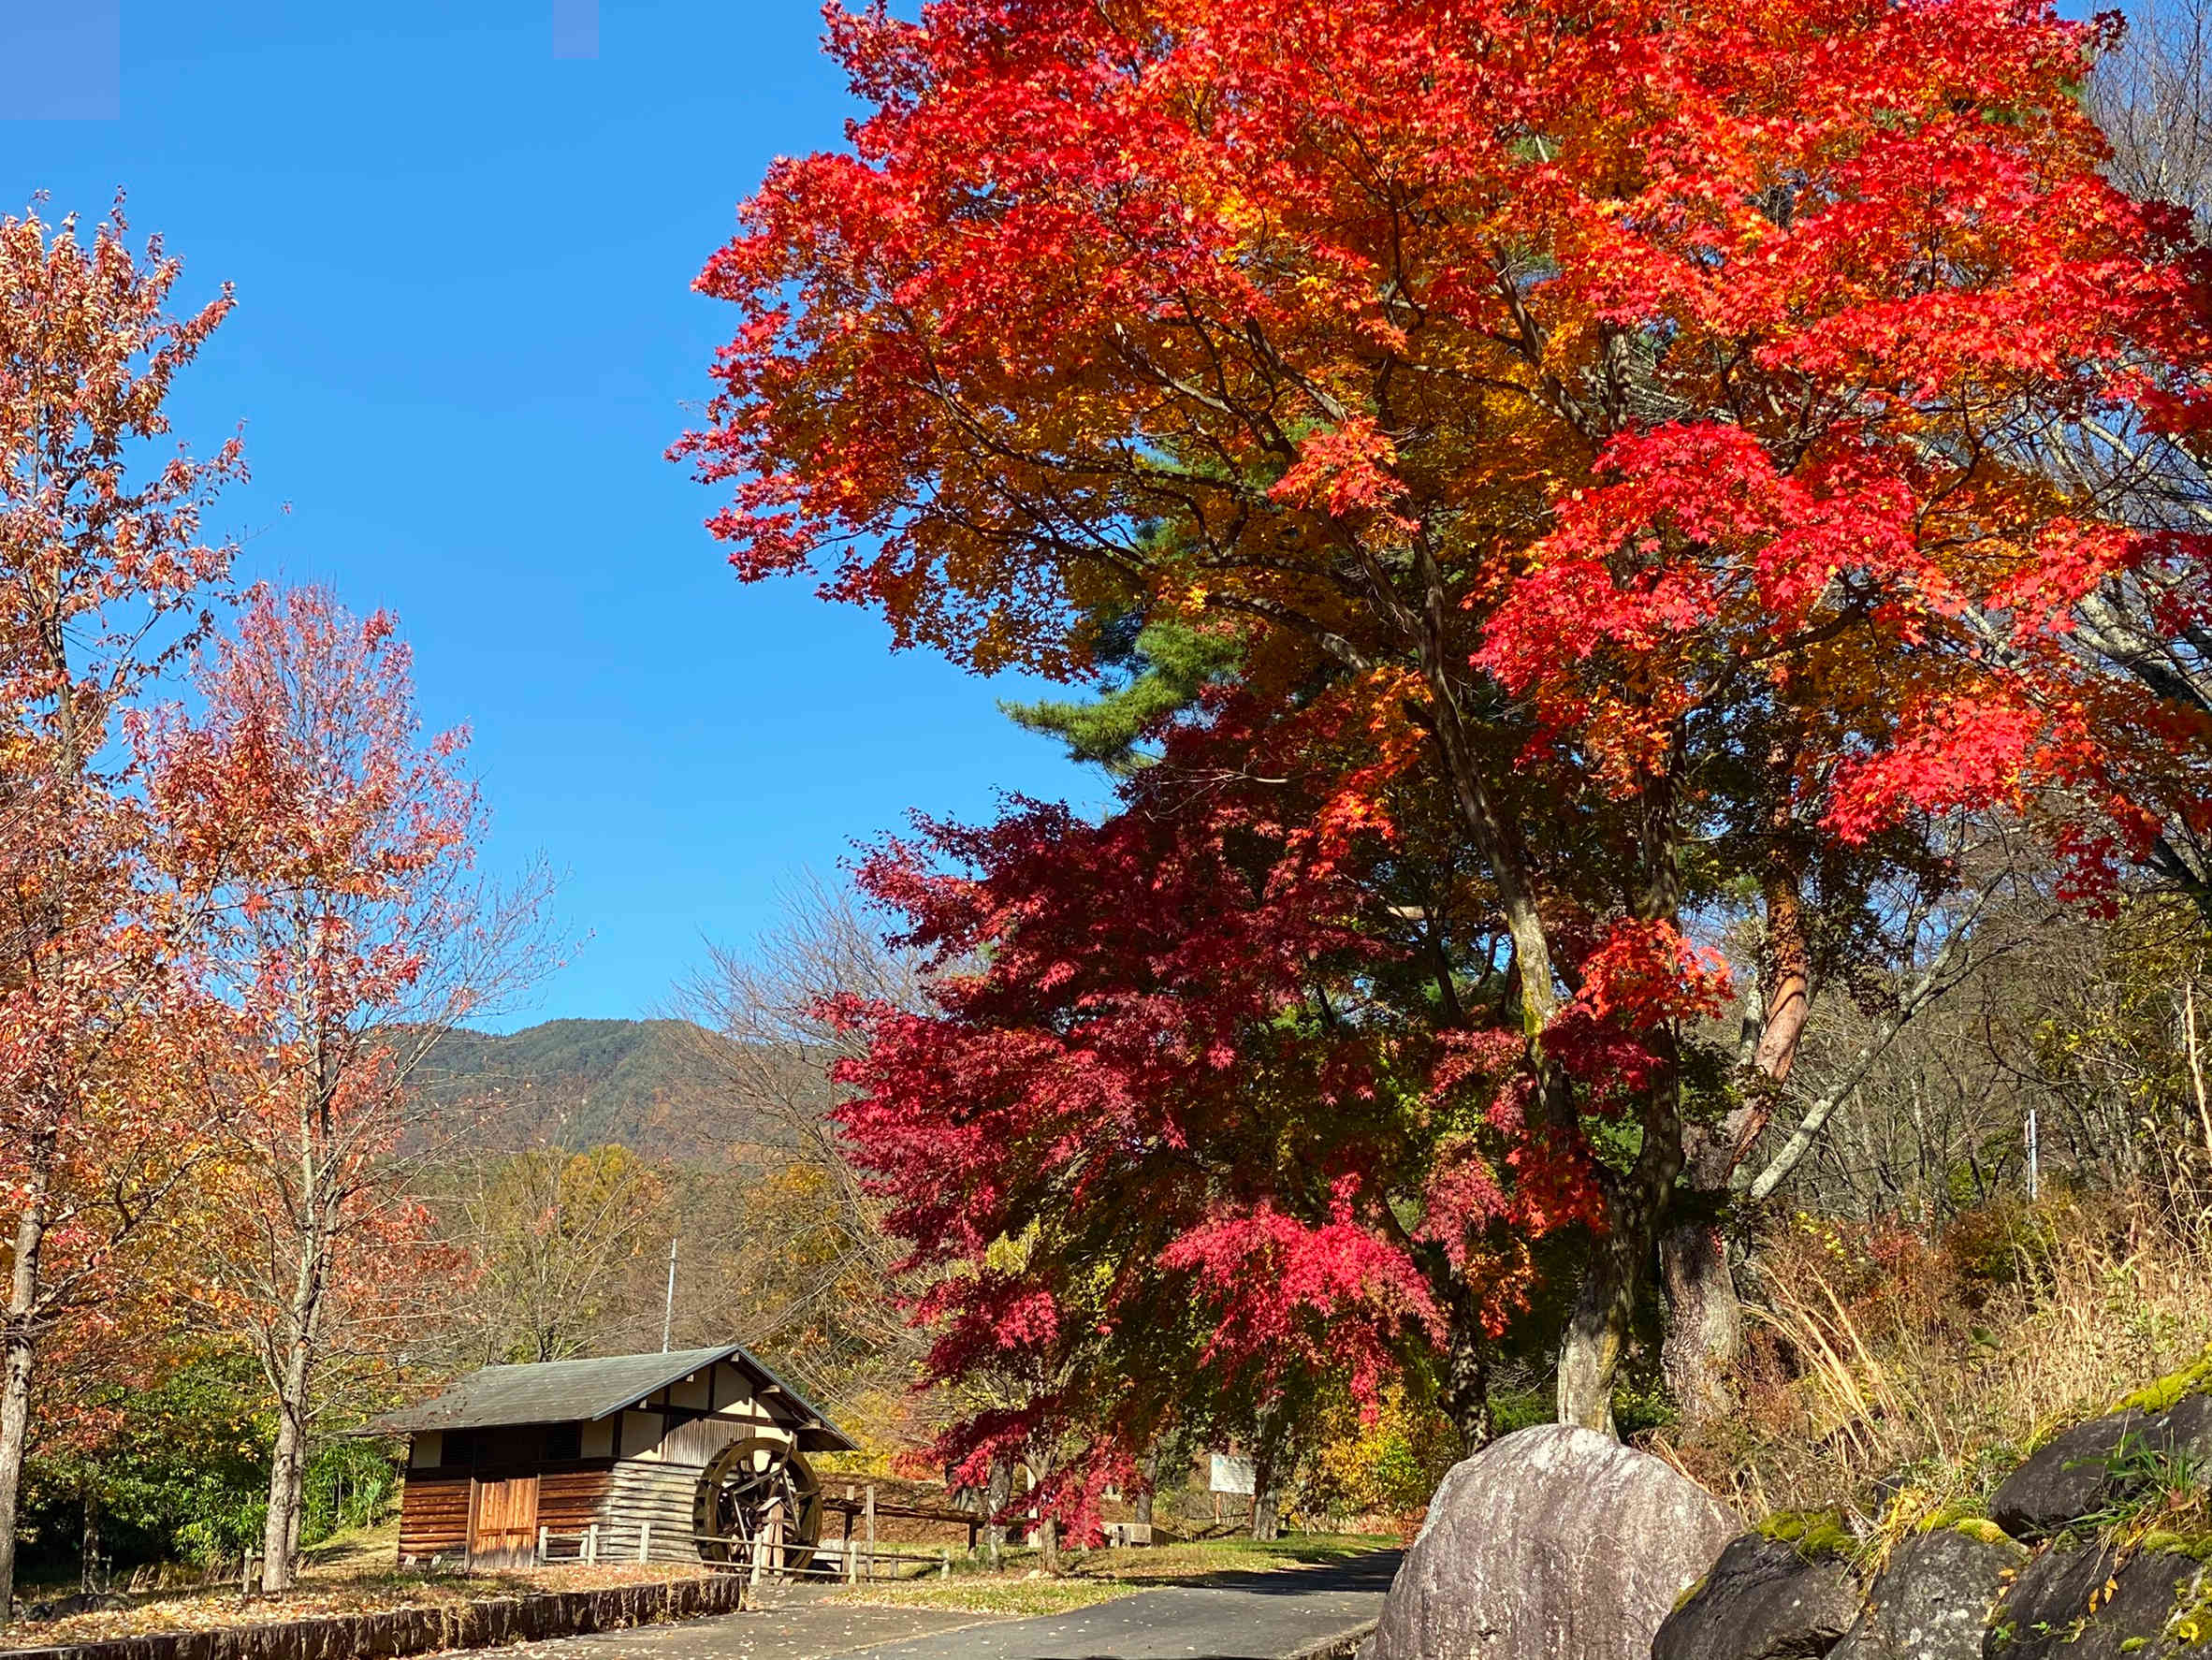
\includegraphics[width=12cm,height=8cm]{kazakosi.jpg}
    \end{center}
    \caption{写真のサンプル
        \label{fig:pm2}
    }
\end{figure}

\chapter{操作例}
システムの操作を実際に示しながら説明する。実際の画面等をここに入れる。

表は次のようにすること。
表の見出しは表の上に配置すること。
本文から必ず参照すること。
表番号は図と同じ要領で付ける。

表 \ref{tab:c1}に示すように、素晴らしいことをやろうとしている。

% ======
%   表
% ======
\begin{table}[htb]
    \caption{セル構成
        \label{tab:c1}
    }
    \begin{center}
        \begin{tabular}{ccc}
            \hline
            Japan  & PDC   & 4 \\
            Europe & GSM   & 3 \\
            USA    & IS-54 & 7 \\
            \hline
        \end{tabular}
    \end{center}
\end{table}

\chapter{結論}
論文で書いたことを簡単にもう一度書いて、主な結果を書く。
新しいことは書かない。
なるべく本文を読まなくてもわかるように書くこと。


% ========
% 参考文献
% ========
\bunken
\begin{thebibliography}{99}
    \bibitem{ref1}
    信州 花子 : 「知的通信と知的符号化」
    電子情報通信学会 情報システム部門 全国大会予稿集
    pp. 1-399 -- 1-401 (1988)

    \bibitem{ref2}
    大下眞二郎,半田志郎,アサノデービッド : 「ディジタル通信」 共立出版 (2005)

    \bibitem{ref3}
    T. Nagano, ``Amazing things that can be done with an eraser,''
    \emph{IEEE Trans. Amazing}, vol. AMA-23, pp. 111-222, Jun. 2009.
\end{thebibliography}

\end{document}
